\subsection[Proceso Interno 09: Actualizar Estado]{Proceso Interno 09: Actualizar Estado de las Partículas}

\subsubsection{Objetivo del Proceso}
El propósito principal de la actividad ``Actualizar Estado de las Partículas'' es consolidar y reflejar oficialmente dentro del objeto \texttt{Simulation} de REBOUND (\texttt{sim}) el nuevo estado físico del sistema gravitacional, incluyendo las posiciones, velocidades, y tiempo de todas las partículas, tras la ejecución de un paso de integración numérica ($dt$) realizado por el integrador seleccionado (por ejemplo, WHFast). Esta actividad asegura que el objeto \texttt{sim} represente de manera coherente el estado del sistema en el nuevo instante de tiempo, preparándolo para las siguientes operaciones en el bucle de simulación, como almacenamiento o visualización.

\subsubsection{Entradas Principales}
\begin{itemize}
    \item \textbf{Referencia al Objeto \texttt{Simulation} (\texttt{sim})}:
    \begin{itemize}
        \item Un puntero o referencia a la instancia del objeto \texttt{Simulation} de REBOUND, recibida inmediatamente después de que la función de integración (por ejemplo, \texttt{sim.integrate~(t\_nuevo)}) haya concluido.
        \item Esta instancia contiene implícitamente:
        \begin{itemize}
            \item Los nuevos valores de posición ($\mathbf{r}_{\text{nuevo}} = [x, y, z]$) y velocidad ($\mathbf{v}_{\text{nuevo}} = [v_x, v_y, v_z]$) de cada partícula, calculados por el integrador y almacenados en \texttt{sim.particles}.
            \item El nuevo tiempo de simulación (\texttt{sim.t} = $t_{\text{nuevo}} = t_{\text{anterior}} + dt$), actualizado por el integrador.
            \item Las masas de las partículas ($m$), que permanecen sin cambios en el contexto estándar del proyecto.
        \end{itemize}
    \end{itemize}
\end{itemize}

\subsubsection{Sub-pasos Secuenciales}
Este apartado es proporcionado para profundizar y describir de forma textual cada paso contenido dentro del diagrama del proceso descrito en la figura~\ref{fig:process_diagram09}
\subsubsection*{1. Finalización del Paso de Integración}
\begin{itemize}
    \item La actividad comienza justo después de que la función de integración de REBOUND (por ejemplo, \texttt{sim.integrate~(t\_nuevo)}) retorna, habiendo completado el cálculo del nuevo estado del sistema para el tiempo $t_{\text{nuevo}}$.
\end{itemize}

\subsubsection*{2. Validar Tiempo de Simulación}
\begin{itemize}
    \item Se verifica que el tiempo interno de la simulación (\texttt{sim.t}) sea igual al tiempo objetivo ($t_{\text{nuevo}} = t_{\text{anterior}} + dt$), asegurando que el integrador ha avanzado correctamente el sistema al instante esperado.
    \item Esta validación confirma la sincronización temporal del estado del sistema.
\end{itemize}

\subsubsection*{3. Verificar Actualización del Estado Físico de las Partículas}
\begin{itemize}
    \item \textbf{Posiciones}:
    \begin{itemize}
        \item Se confirma que las posiciones de todas las partículas en \texttt{sim.particles} han sido actualizadas por el integrador a los nuevos valores ($\mathbf{r}_{\text{nuevo}} = [x, y, z]$), correspondientes al tiempo $t_{\text{nuevo}}$.
    \end{itemize}
    \item \textbf{Velocidades}:
    \begin{itemize}
        \item Se verifica que las velocidades de todas las partículas en \texttt{sim.particles} han sido actualizadas a los nuevos valores ($\mathbf{v}_{\text{nuevo}} = [v_x, v_y, v_z]$), calculados por el integrador.
    \end{itemize}
    \item \textbf{Masas}:
    \begin{itemize}
        \item En el contexto de este proyecto, donde no se implementa la modificación dinámica de masas durante la integración estándar, se confirma que las masas de las partículas ($m$) en \texttt{sim.particles} permanecen sin cambios respecto al paso anterior.
    \end{itemize}
    \item Estas verificaciones aseguran que el estado físico del sistema, almacenado en \texttt{sim.particles}, refleja correctamente los resultados del paso de integración.
\end{itemize}

\subsubsection*{4. Validación de Coherencia (Opcional)}
\begin{itemize}
    \item \textbf{Conservación de Energía}:
    \begin{itemize}
        \item Opcionalmente, se calcula la energía total del sistema (cinética más potencial) en el nuevo estado y se compara con el estado anterior para verificar una conservación aproximada, dentro de los límites de precisión del integrador (por ejemplo, WHFast).
    \end{itemize}
    \item \textbf{Conservación de Momento Angular}:
    \begin{itemize}
        \item Opcionalmente, se calcula el momento angular total y se verifica su conservación aproximada, asegurando que el integrador no ha introducido errores significativos.
    \end{itemize}
    \item \textbf{Coherencia General}:
    \begin{itemize}
        \item Se realiza una comprobación general para asegurar que el estado físico es consistente (por ejemplo, posiciones y velocidades son valores numéricos válidos, no \texttt{NaN} ni infinitos).
    \end{itemize}
    \item Estas validaciones son opcionales y pueden omitirse en implementaciones estándar si se confía en la robustez del integrador.
\end{itemize}

\subsubsection*{5. Actualización del Estado Computacional}
\begin{itemize}
    \item \textbf{Variables Auxiliares (Si Existen)}:
    \begin{itemize}
        \item Se actualizan cualquier variable auxiliar interna de \texttt{sim} que pueda ser utilizada por REBOUND (por ejemplo, acumuladores para métricas de error o estados intermedios del integrador).
    \end{itemize}
    \item \textbf{Sincronización de Coordenadas (Si Aplica)}:
    \begin{itemize}
        \item Si el integrador utiliza múltiples sistemas de coordenadas (por ejemplo, Jacobi para cálculos internos y baricéntricas para reporte), se sincronizan las representaciones para asegurar que el estado reportado en \texttt{sim.particles} esté en el sistema esperado por los procesos posteriores.
    \end{itemize}
    \item Estas operaciones garantizan que el estado computacional de \texttt{sim} esté alineado con el estado físico.
\end{itemize}

\subsubsection*{6. Estado Coherente del Sistema}
\begin{itemize}
    \item En este punto, el objeto \texttt{sim} representa de manera consistente el estado del sistema en el tiempo $t_{\text{nuevo}}$, con \texttt{sim.t} actualizado y \texttt{sim.particles} conteniendo las nuevas posiciones, velocidades, y masas (sin cambios).
\end{itemize}

\subsubsection*{7. Listo para la Siguiente Acción}
\begin{itemize}
    \item La instancia \texttt{sim}, con su estado interno completamente actualizado, está preparada para las operaciones siguientes en el bucle principal de simulación, como almacenar el estado, verificar tiempos de visualización, o ejecutar otro paso de integración.
\end{itemize}

\subsubsection{Lógica Interna y Decisiones}
\begin{itemize}
    \item \textbf{Validación del Tiempo}:
    \begin{itemize}
        \item La verificación de que \texttt{sim.t} = $t_{\text{nuevo}}$ es una decisión implícita que asegura la sincronización temporal. Si no se cumple, podría indicar un error en el integrador, pero esto es manejado por REBOUND internamente.
    \end{itemize}
    \item \textbf{Validaciones Opcionales}:
    \begin{itemize}
        \item La decisión de realizar verificaciones de conservación (energía, momento angular) o coherencia general depende de los requisitos de robustez del sistema. Si se implementan, introducen bifurcaciones donde un fallo (por ejemplo, energía no conservada) podría desencadenar un manejo de errores, como lanzar una excepción.
    \end{itemize}
    \item \textbf{Sincronización de Coordenadas}:
    \begin{itemize}
        \item La necesidad de sincronizar sistemas de coordenadas depende de la configuración del integrador y los requisitos de los procesos posteriores. Esta decisión es condicional y se basa en el estado interno de \texttt{sim}.
    \end{itemize}
    \item \textbf{Ausencia de Transformación Directa}:
    \begin{itemize}
        \item No hay transformación de datos en esta actividad, ya que el integrador ya ha actualizado el estado en \texttt{sim}. La lógica se centra en verificar y consolidar ese estado, con decisiones orientadas a la validación y sincronización.
    \end{itemize}
\end{itemize}

\subsubsection{Manejo de Datos Específico}
\begin{itemize}
    \item \textbf{Datos de Entrada}:
    \begin{itemize}
        \item Referencia al objeto \texttt{Simulation} (\texttt{sim}) post-integración, que contiene implícitamente:
        \begin{itemize}
            \item Nuevo tiempo (\texttt{sim.t} = $t_{\text{nuevo}}$).
            \item Nuevas posiciones y velocidades en \texttt{sim.particles}.
            \item Masas sin cambios en \texttt{sim.particles}.
        \end{itemize}
    \end{itemize}
    \item \textbf{Datos Intermedios}:
    \begin{itemize}
        \item Resultados de las verificaciones (por ejemplo, valores de energía o momento angular, si se calculan).
        \item Estado de variables auxiliares o sistemas de coordenadas sincronizados, si aplica.
    \end{itemize}
    \item \textbf{Datos de Salida}:
    \begin{itemize}
        \item La instancia \texttt{sim} con su estado interno consolidado, representando el sistema en $t_{\text{nuevo}}$.
    \end{itemize}
\end{itemize}

\subsubsection{Salidas Principales}
\begin{itemize}
    \item \textbf{Instancia \texttt{sim} Actualizada}:
    \begin{itemize}
        \item La referencia al objeto \texttt{Simulation} (\texttt{sim}), con su estado interno (tiempo \texttt{sim.t}, posiciones y velocidades en \texttt{sim.particles}) consolidado y coherente para el tiempo $t_{\text{nuevo}}$, lista para las siguientes acciones en el bucle de simulación.
    \end{itemize}
\end{itemize}

\subsubsection{Interacciones Internas}
\begin{itemize}
    \item \textbf{Con la API de REBOUND}:
    \begin{itemize}
        \item Depende directamente de la función de integración (por ejemplo, \texttt{sim.integrate~()}), que modifica el estado interno de \texttt{sim} (\texttt{sim.t}, \texttt{sim.particles}) antes de que esta actividad comience.
        \item Accede a las propiedades de \texttt{sim} (como \texttt{sim.t} y \texttt{sim.particles}) para verificar el estado actualizado.
    \end{itemize}
    \item \textbf{Con el Estado Interno de \texttt{sim}}:
    \begin{itemize}
        \item Inspecciona y, si es necesario, sincroniza las estructuras internas de \texttt{sim}, incluyendo el tiempo, las partículas, y posibles variables auxiliares.
    \end{itemize}
    \item \textbf{Con el Flujo de Simulación}:
    \begin{itemize}
        \item Se integra en el bucle principal de simulación, actuando como el punto donde se consolida el estado tras cada paso de integración, preparando \texttt{sim} para procesos como almacenamiento o visualización.
    \end{itemize}
\end{itemize}
\newpage
\subsubsection{Diagrama del Proceso}
\begin{figure}[H]
    \centering
    \adjustbox{max width=\textwidth, max height=0.9\textheight}{%
        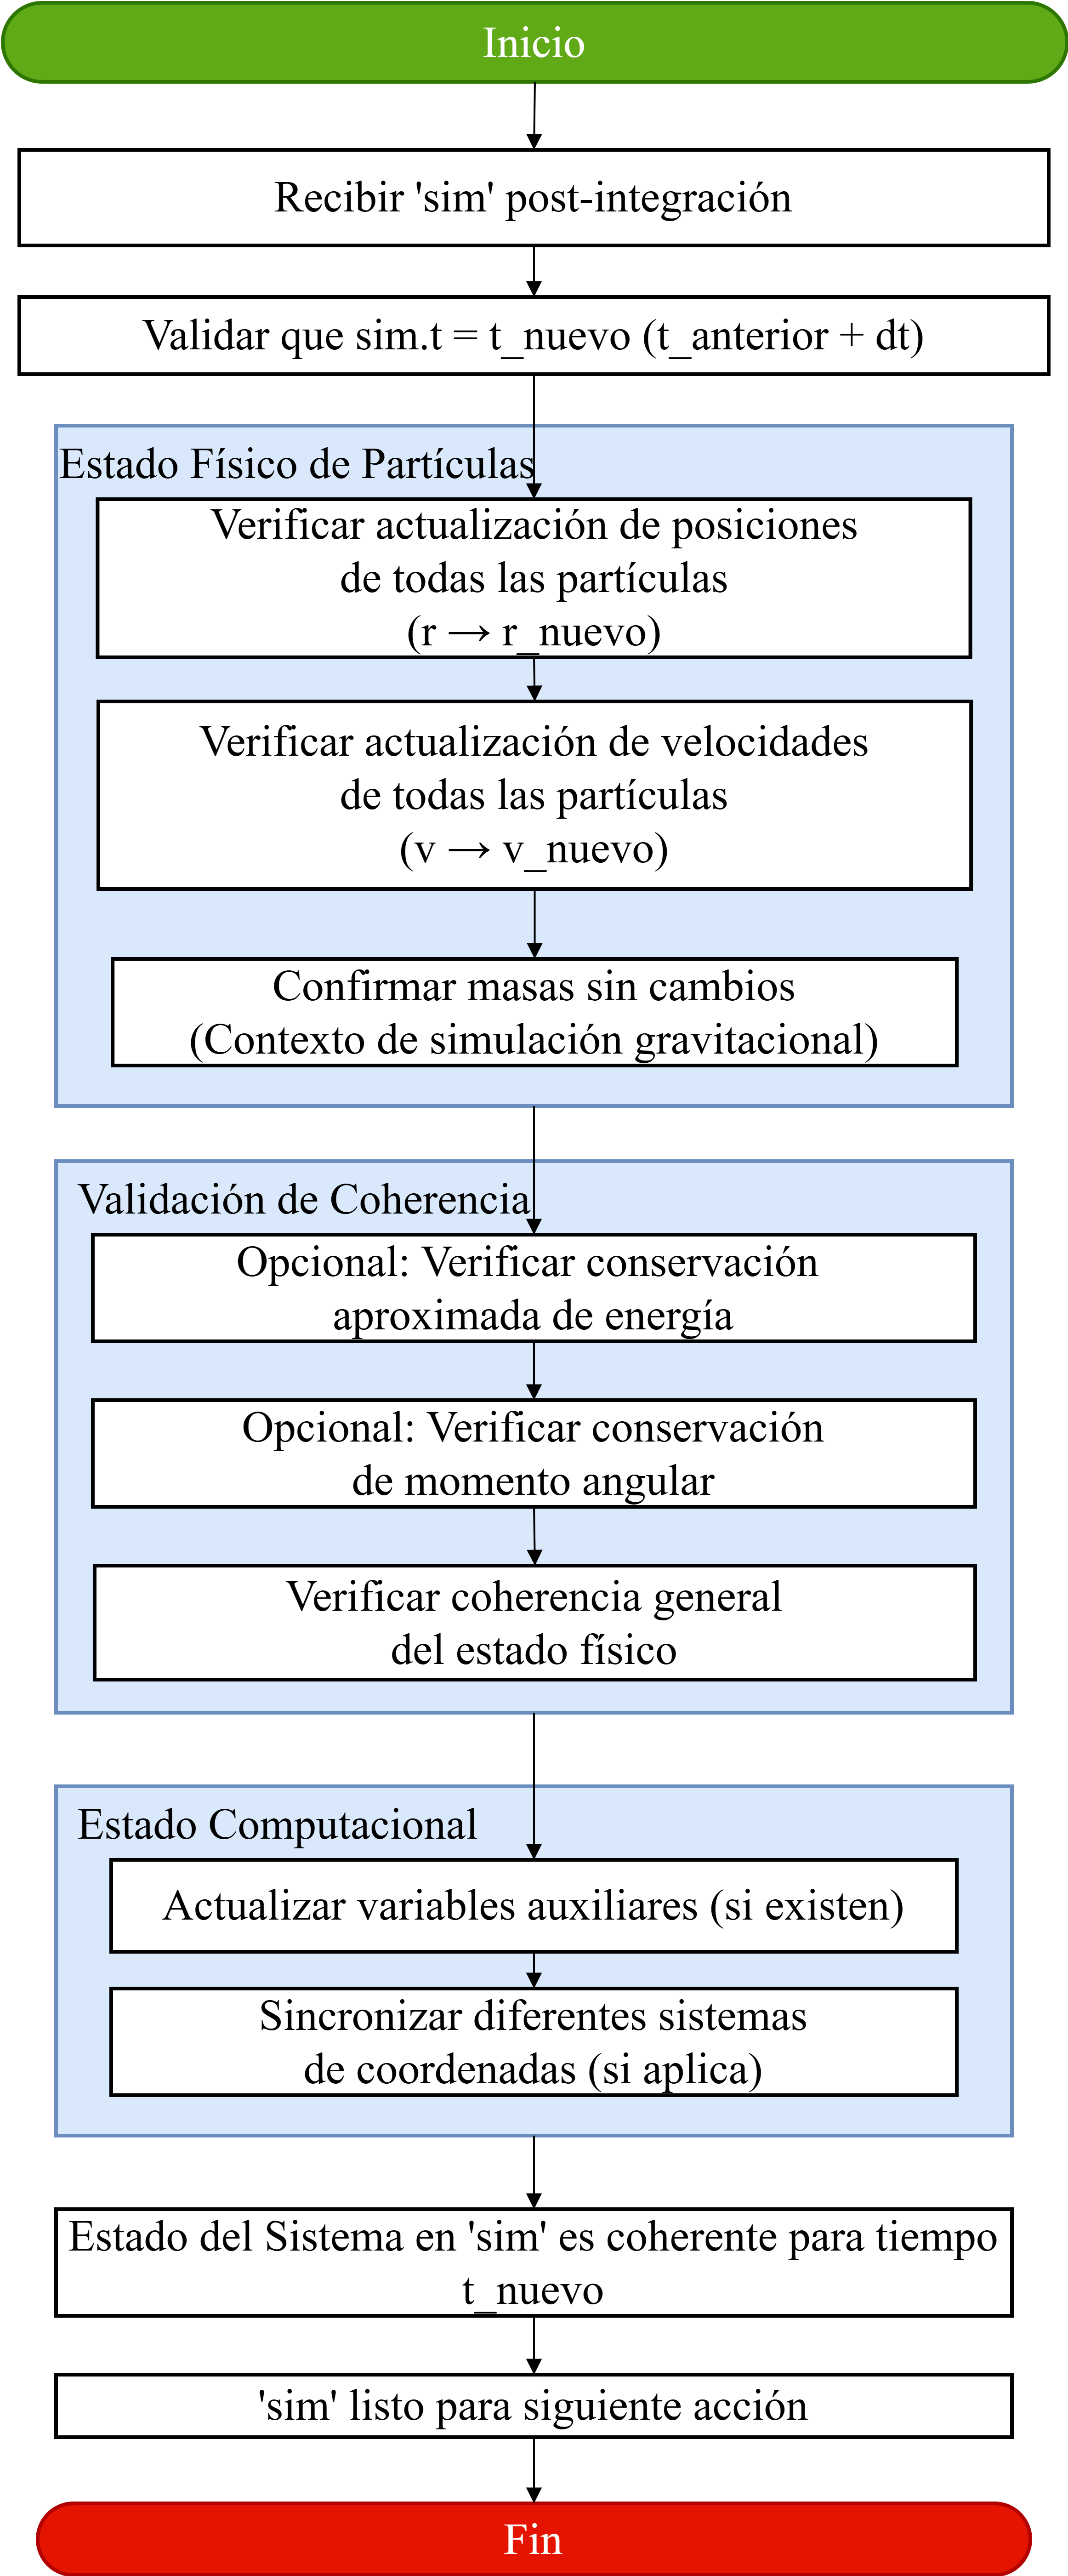
\includegraphics{img/Analisis/DiagramaProcesos/DiagramaProceso09_ActualizarEstado.png}
    }
        \caption{Diagrama de Proceso Interno 09: Actualizar Estado}%
    \label{fig:process_diagram09}
\end{figure}
\newpage